\chapter{Návrh testov pre systém Fitcrack}
K~návrhu testov pre systém Fitcrack potrebujeme poznať:
\begin{itemize}
	\item architektúru systému Fitcrack~\ref{Fitcrack},
	\item moduly, ktoré budú testované~\ref{tests_moduls},
	\item kedy budú ktoré moduly testované~\ref{test_design},
	\item spôsoby testovania~\ref{testing_levels},
\end{itemize}
Fitcrack pozostáva z niekoľkých častí, tak ako sú navrhnuté v systéme BOINC~\cite{boincintro}.
V mojej práci som sa rozhodol testovať s použitím zdrojových kódov, keďže nemám k dispozícii kompletnú špecifikáciu systému, alebo jeho komponentov. 
Tvorba testov vychádza z požiadaviek na konkrétny komponent.
U modulu generátor a asimilátor, ktorých činnosť je popísaná pseudokódom~\ref{alg:generator} a~\ref{alg:asimilator} som sa rozhodol vytvoriť CFG a vytvoriť požiadavky na základe prechodu grafu. 
Na nájdenie primárnych ciest grafu som použil nástroj Prime Path Coverage\footnote{\url{https://github.com/heshenghuan/Prime-Path-Coverage}}.

Podľa Google blogu o testovaní\footnote{\url{http://blog.codepipes.com/testing/software-testing-antipatterns.html}} spadajú do kategórie integračných testov~\ref{integration_tests}, no každý test testuje iba jediný modul, takže budem používať názov testovanie modulov.

Pre implementáciu bol vybraný unittest\footnote{\url{https://docs.python.org/3.6/library/unittest.html}} framework z čoho vyplýva, že testy budú implementované v jazyku Python3.
Moduly by mali byť testovateľné samostatne, takže každý modul bude testovaný inou triedou.

Prístup do databáze je pomocou frameworku SQL ALchemy\footnote{\url{https://www.sqlalchemy.org/}}.
Je to jeden z najpouživanejších frameworkov v jazyku Python, dovoľuje používať ORM (Object Relation Mapper)\footnote{\url{https://en.wikipedia.org/wiki/Object-relational_mapping}} a využíva ho aj API, takže ho nebude potrebné inštalovať.


\section{Návrh testov pre modul generátor}
Generátor má na starosti generovanie nových úloh pre klientov a rozdeľovanie nových, či neúspešne dokončených úloh. 
Komunikuje výhradne s databázou, beží v nekonečnom cykle, kde periodicky kontroluje bežiace balíky a ak je to potrebné generuje nové úlohy, alebo prerozdeľuje neúspešne dokončené úlohy.
Generátor dopĺňa TLV slovník~\ref{from_server}, ktorý sa vytvára pri pridaní nového balíčka.
Doplnený TLV slovník je určený pre runner, ktorý podľa neho vie o akú úlohu sa jedná a aké parametre má poslať Hashcat-u.

Pre testovanie bol pôvodný zámer implementovať pokrytie primárny ciest~\ref{kriteria_cfg}, no po vygenerovaní všetkých primárnych ciest pomocou vyššie spomínaného program Prime path coverage bolo od tohto zámeru upustené, hlavne kvôli rozsahu, keďže počet primárnych ciest je 777.
Nakoniec som uznal za vhodné vybrať kritérium pokrytia všetkých uzlov (node coverage).

Kontrolované bude či generátor vytvára správne záznamy v databáza, či správne mení hodnoty existujúcich záznamov v databáze a čo správne vytvára TLV konfiguračne súbory~\ref{from_server}.

\begin{figure}[h]
	\centering
	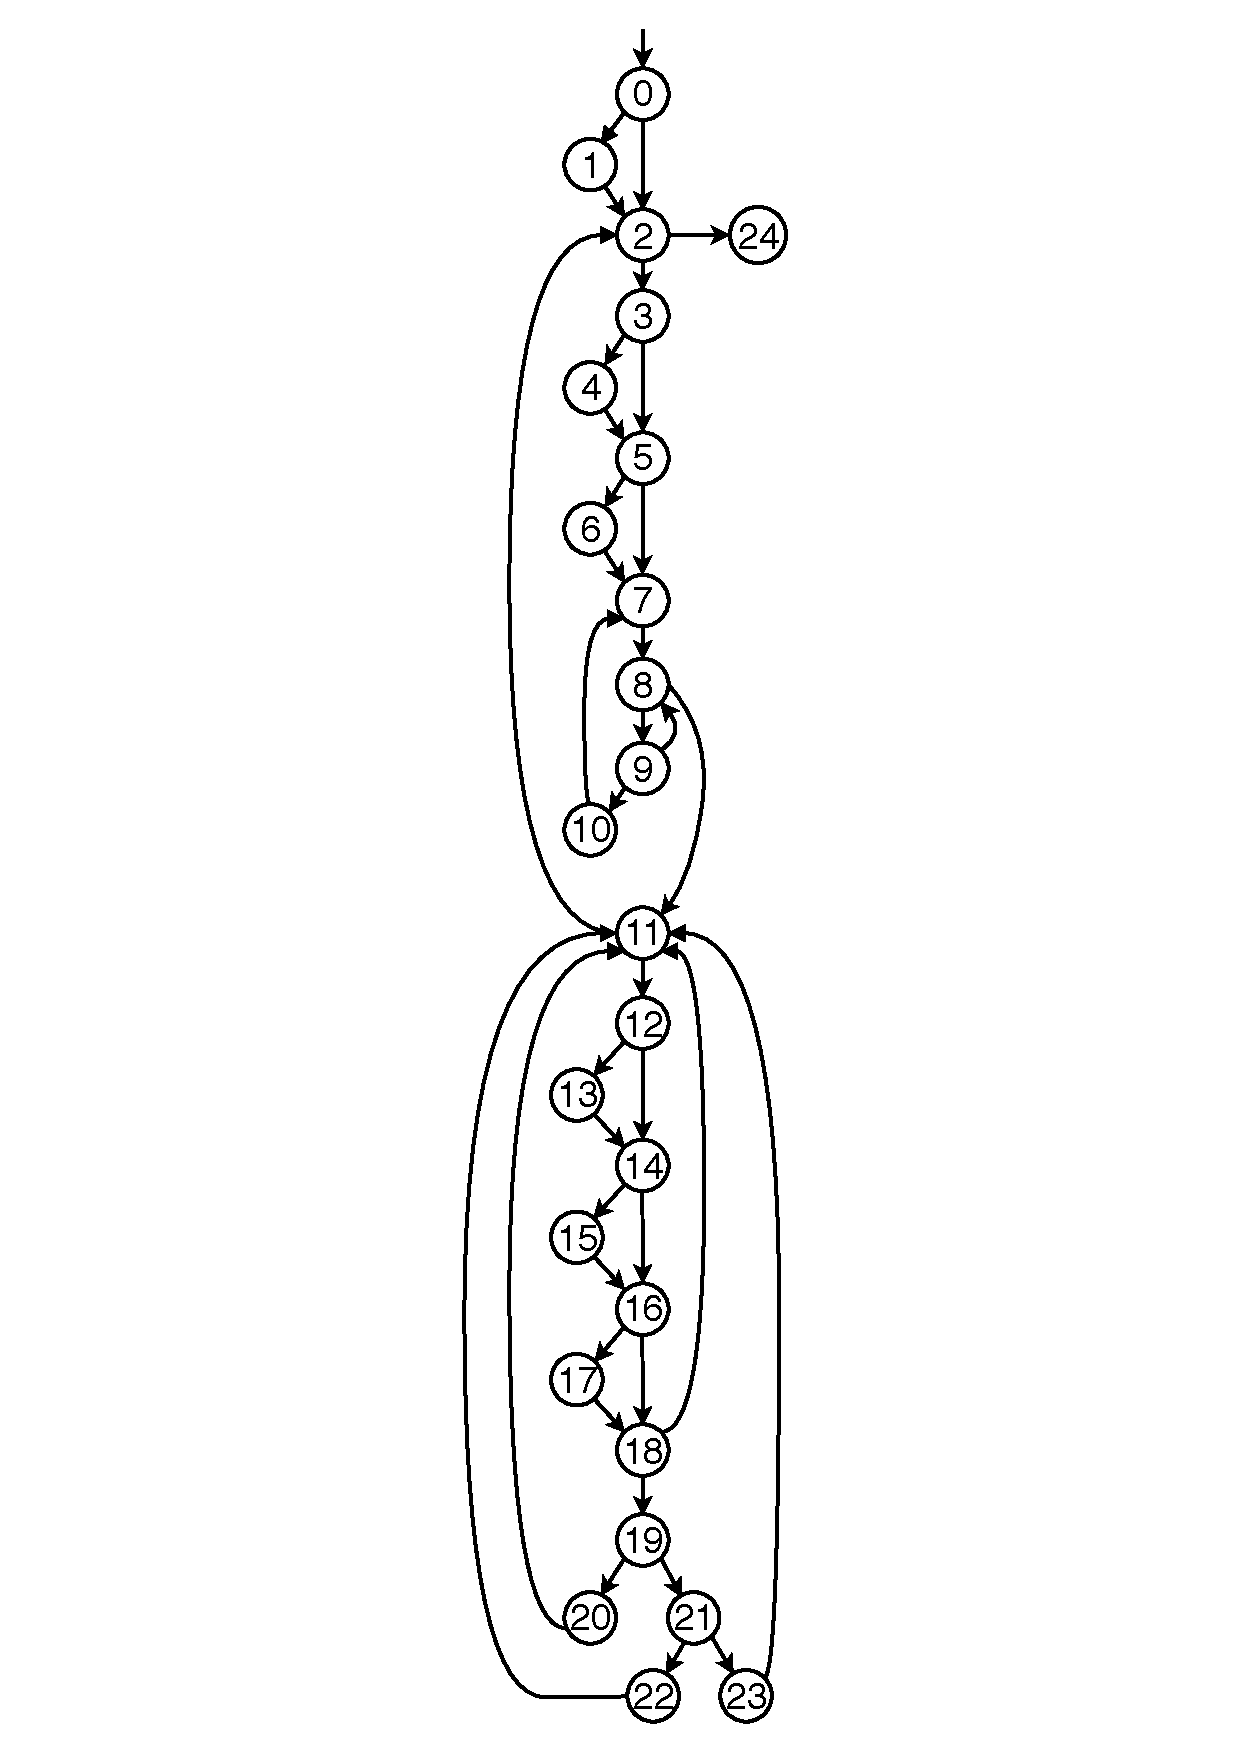
\includegraphics[height=0.7\paperheight]{obrazky/cfg_generator.pdf}
	\caption{CFG generátora vytvorené z pseudokódu~\ref{alg:generator}.}
	\label{fig:cfg_gen}
\end{figure}


\section{Návrh testov pre modul asimilátor}
\label{navrh_asim}
Asimilátor je podobne ako generátor serverový modul a komunikuje výhradne pomocou databázy.
Jeho funkcia spočíva v spracovávaní výsledkov úloh od klienta.
Narozdiel od generátora je asimilátor volaný Boinc-om, keď je v databáze validovaný výsledok úlohy, takže pred každým testom je potrebné pripraviť záznamy tabuliek databázy so správnymi hodnotami, aby bol asimilátor zavolaný.
Vstupný bod assimilátora je funkcia \texttt{assimilate\_handler()}\footnote{\url{https://boinc.berkeley.edu/trac/wiki/AssimilateIntro}}.

Asimilátor je jednoduchší modul, ako generátor, takže je možné dosiahnúť pokrytie všetkých primárnych ciest.
CFG asimilátora je zobrazený na obrázku~\ref{fig:cfg_asim}.
Počet primárnych ciest je 14:
\begin{center}
	\begin{verbatim}
		[0, 6, 14, 15]
		[0, 6, 14, 16]
		[0, 1, 5, 14, 15]
		[0, 1, 5, 14, 16]
		[0, 6, 7, 8, 14, 15]
		[0, 6, 7, 8, 14, 16]
		[0, 6, 7, 13, 14, 15]
		[0, 6, 7, 13, 14, 16]
		[0, 1, 2, 3, 4, 14, 15]
		[0, 1, 2, 3, 4, 14, 16]
		[0, 6, 7, 9, 10, 12, 14, 15]
		[0, 6, 7, 9, 10, 12, 14, 16]
		[0, 6, 7, 9, 10, 11, 12, 14, 15]
		[0, 6, 7, 9, 10, 11, 12, 14, 16]
	\end{verbatim}
\end{center}

Pri testovaní asimilátora bude potrebné kontrolovať aké zmeny boli prevedené v databázi a či je daná úloha úspešne asimilovaná.

\begin{figure}[h]
	\centering
	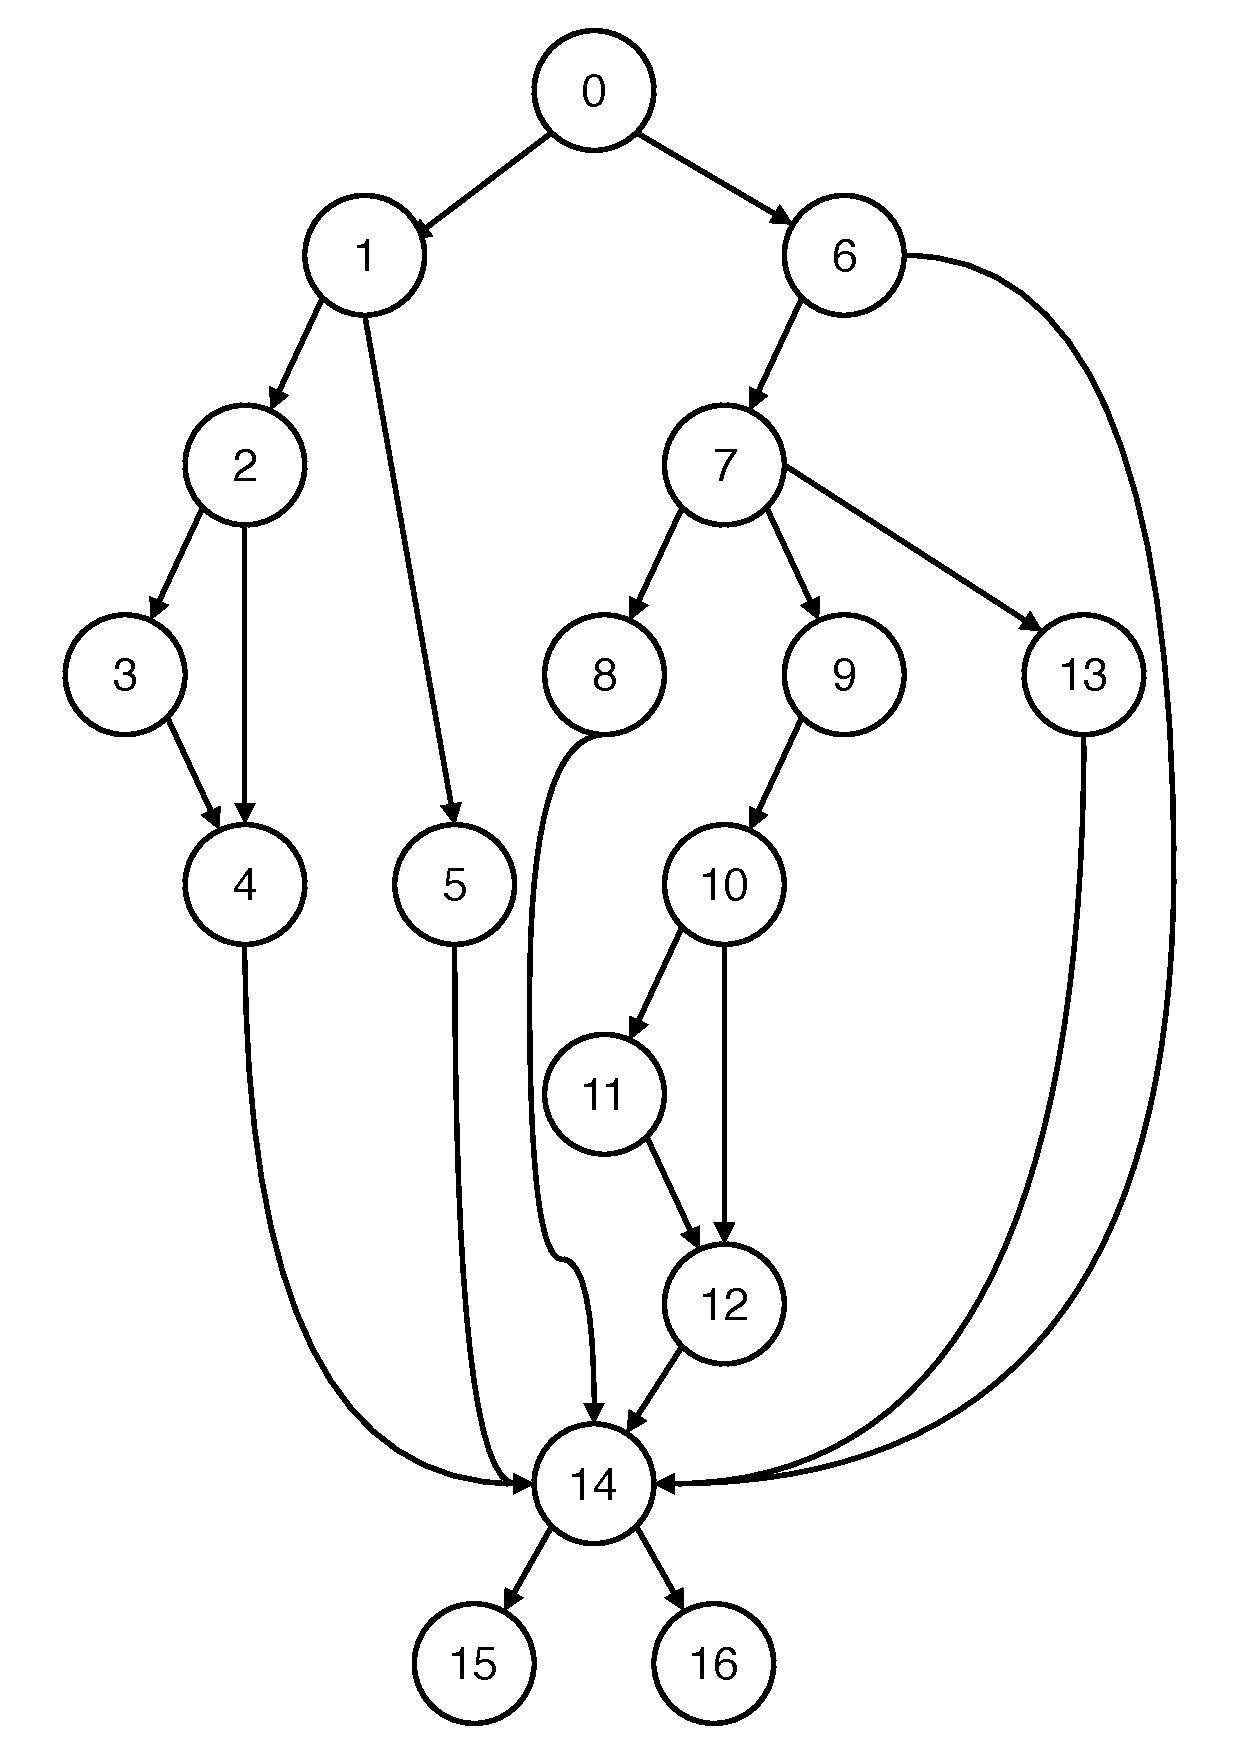
\includegraphics[height=0.7\paperheight]{obrazky/cfg_asimilator.pdf}
	\caption{CFG asimilátora vytvorené z pseudokódu~\ref{alg:asimilator}.}
	\label{fig:cfg_asim}
\end{figure}


\section{Návrh testov pre modul runner}
Runner má za úlohu spúštať Hashcat podľa konfiguračného TLV súboru~\ref{from_server}, kontrolovať priebeh výpočtu Hashcatu a keď výpočeť skončí runner by mal vytvoriť výstupný súbor s výsledkami úlohy~\ref{from_client}.

Testovanie runnera je potrebné rozdeliť na 2 časti: testovanie, že runner spúšťa hashcat so správnymi parametrami a testovanie, že runner vytvára správne výstupné súbory podľa výstupu Hashcatu.
Neexistuje presná špecifikácia runnera, takže nie je možné použiť žiadnu z metód popisovaných v kapitole~\ref{requirements_based_testing}, no je možné sa inšprovať testovaním založenom na vstupných doménach~\ref{vstupne_domeny}, kedže nepoznáme vnútornú špecifikáciu, ale vieme ako sa ma správať pre rôzne kategórie vstupov a výstupov.

Aby sme mohli kontrolovať správnosť argumentov s ktorými runner spúšťa Hashcat a mohli kontrolovať výstup Hashcatu je potrebné vytvoriť náhradu za Hashcat.
V našom prípade to bude mock~\ref{mock}, keďže nesprávne argumenty môžu spôsobiť zlyhanie testu a náhrade bude vraciať rôzne výstupy v závislosti na vstupe.


\section{Návrh testov pre API}
API z časti nahradzuje funkciu webAdmina, vzhľadom nato, že je cez neho možné ovládať všetky časti systému Fitcrack ako pridávanie nových balíčkov, hosťov, spúšťanie, pozastavenie crackovania, alebo celého projektu cez BOINC ovládacie prvky a iné.
API je rozdelené do endpointov, kde každý z nich má na starosti inú časť systému~\ref{API} a každý endpoint má rôzne vstupné parametre na ktoré sa dá aplikovať testovanie založené na vstupných doménach~\ref{vstupne_domeny}.
Odpovede na dotazy v API budú vo formáte \texttt{json}, takže pre každý objekt používaný v databázi a dotazovaný pomocou API bude potrebné implementovať ekvivalentný prevod aký robí API.
